\documentclass[11pt]{article}

% --- Encoding and fonts ---
\usepackage[utf8]{inputenc}
\usepackage[T1]{fontenc}
\usepackage{lmodern}

% --- Layout ---
\usepackage[a4paper,margin=1in]{geometry}
\usepackage{microtype}
\setlength{\parskip}{0.4em}
\setlength{\parindent}{0pt}

% --- Math, tables, graphics ---
\usepackage{amsmath,amssymb}
\usepackage{booktabs}
\usepackage{array}
\usepackage{tabularx}
\newcolumntype{Y}{>{\raggedright\arraybackslash}X}
\usepackage{alltt}
\usepackage{tikz}
\usetikzlibrary{arrows.meta,positioning}

% --- Links ---
\usepackage[hidelinks]{hyperref}

% --- Raw-unicode coverage (markdown source uses literal unicode in prose/tables) ---
\usepackage{newunicodechar}
\newunicodechar{−}{$-$}\newunicodechar{×}{$\times$}\newunicodechar{÷}{$\div$}
\newunicodechar{±}{$\pm$}\newunicodechar{≈}{$\approx$}\newunicodechar{≠}{$\neq$}
\newunicodechar{≤}{$\leq$}\newunicodechar{≥}{$\geq$}\newunicodechar{∈}{$\in$}
\newunicodechar{∞}{$\infty$}\newunicodechar{→}{$\to$}\newunicodechar{↦}{$\mapsto$}
\newunicodechar{⊗}{$\otimes$}\newunicodechar{⊕}{$\oplus$}\newunicodechar{∂}{$\partial$}
\newunicodechar{∇}{$\nabla$}\newunicodechar{∑}{$\sum$}\newunicodechar{∫}{$\int$}
\newunicodechar{√}{$\sqrt{}$}\newunicodechar{α}{$\alpha$}\newunicodechar{β}{$\beta$}
\newunicodechar{γ}{$\gamma$}\newunicodechar{δ}{$\delta$}\newunicodechar{ε}{$\varepsilon$}
\newunicodechar{η}{$\eta$}\newunicodechar{θ}{$\theta$}\newunicodechar{λ}{$\lambda$}
\newunicodechar{μ}{$\mu$}\newunicodechar{ν}{$\nu$}\newunicodechar{ξ}{$\xi$}
\newunicodechar{π}{$\pi$}\newunicodechar{ρ}{$\rho$}\newunicodechar{σ}{$\sigma$}
\newunicodechar{τ}{$\tau$}\newunicodechar{φ}{$\varphi$}\newunicodechar{χ}{$\chi$}
\newunicodechar{ψ}{$\psi$}\newunicodechar{ω}{$\omega$}\newunicodechar{Γ}{$\Gamma$}
\newunicodechar{Δ}{$\Delta$}\newunicodechar{Λ}{$\Lambda$}\newunicodechar{Σ}{$\Sigma$}
\newunicodechar{Φ}{$\Phi$}\newunicodechar{Ψ}{$\Psi$}\newunicodechar{Ω}{$\Omega$}
\newunicodechar{ℏ}{$\hbar$}\newunicodechar{ℓ}{$\ell$}\newunicodechar{ℝ}{$\mathbb{R}$}
\newunicodechar{ℂ}{$\mathbb{C}$}\newunicodechar{ℕ}{$\mathbb{N}$}\newunicodechar{ℤ}{$\mathbb{Z}$}
\newunicodechar{…}{\ldots}\newunicodechar{—}{---}\newunicodechar{–}{--}
\newunicodechar{‘}{`}\newunicodechar{’}{'}\newunicodechar{“}{``}\newunicodechar{”}{''}
\newunicodechar{·}{$\cdot$}\newunicodechar{↔}{$\leftrightarrow$}\newunicodechar{⟹}{$\Longrightarrow$}
\newunicodechar{⟸}{$\Longleftarrow$}\newunicodechar{⟺}{$\Longleftrightarrow$}
\newunicodechar{←}{$\leftarrow$}\newunicodechar{⇒}{$\Rightarrow$}\newunicodechar{⇐}{$\Leftarrow$}
\newunicodechar{⇔}{$\Leftrightarrow$}\newunicodechar{≡}{$\equiv$}\newunicodechar{≅}{$\cong$}
\newunicodechar{≃}{$\simeq$}\newunicodechar{∝}{$\propto$}\newunicodechar{∀}{$\forall$}
\newunicodechar{∃}{$\exists$}\newunicodechar{∅}{$\emptyset$}\newunicodechar{¬}{$\neg$}
\newunicodechar{∧}{$\wedge$}\newunicodechar{∨}{$\vee$}\newunicodechar{⊥}{$\perp$}
\newunicodechar{∥}{$\parallel$}\newunicodechar{∘}{$\circ$}\newunicodechar{•}{$\bullet$}
\newunicodechar{⊆}{$\subseteq$}\newunicodechar{⊂}{$\subset$}\newunicodechar{⊇}{$\supseteq$}
\newunicodechar{⊃}{$\supset$}\newunicodechar{∩}{$\cap$}\newunicodechar{∪}{$\cup$}
\newunicodechar{∖}{$\setminus$}\newunicodechar{⟨}{$\langle$}\newunicodechar{⟩}{$\rangle$}
\newunicodechar{†}{$\dagger$}\newunicodechar{′}{$'$}\newunicodechar{⊤}{$\top$}
\newunicodechar{⊨}{$\models$}\newunicodechar{⊢}{$\vdash$}\newunicodechar{∎}{$\blacksquare$}
\newunicodechar{☆}{$\star$}\newunicodechar{★}{$\star$}\newunicodechar{§}{\S}
\newunicodechar{²}{\textsuperscript{2}}\newunicodechar{³}{\textsuperscript{3}}
\newunicodechar{¹}{\textsuperscript{1}}\newunicodechar{₀}{\textsubscript{0}}
\newunicodechar{₁}{\textsubscript{1}}\newunicodechar{₂}{\textsubscript{2}}
\newunicodechar{₃}{\textsubscript{3}}\newunicodechar{ₙ}{\textsubscript{n}}
\newunicodechar{✓}{\checkmark}\newunicodechar{µ}{$\mu$}

\title{An Audited Human-AI Loop for Trustworthy Lean Formalization:\\
Axiom-Budget Auditing, a Goal-Directed State Report, and a Conditional General-Relativity Case Study}
\author{Paweł Kapłański}
\date{2026-06-21}

\begin{document}
\maketitle

\begin{abstract}
\noindent
AI can now write mathematics and code faster than humans can vet it, and in a proof assistant a
proof that merely compiles is not enough: the load-bearing content can hide in a declared axiom, and
"it builds, with no \texttt{sorry}" cannot distinguish a sound development from one resting on a false,
vacuous, or over-strong assumption. We present a human-directed, two-model formalization loop built
around that gap. A coding agent (Claude Code) writes Lean 4 / Mathlib and self-corrects against the
compiler; an independent model (GPT-5.5-Pro) adversarially reviews the \emph{design} rather than the
syntax; and a human controls scope and premises. The soundness contribution is the audit that wraps
the loop: a continuously-enforced \emph{axiom budget} that classifies every result as proved /
conditional / cited and can only ratchet down; a \emph{vacuity lint} and a *hypothesis ledger /
redundancy probe* that extend the audit from declared axioms to a theorem's local hypotheses; a
\emph{goal-directed track-state report} that turns the audit into the loop's steering signal; and a
link-checked blueprint from prose to kernel-checked declarations. We assess the division of labour
with a small controlled \emph{instrument ablation} (seeded faults run past each instrument): the
structural instruments catch structural faults, while only the independent reviewer diagnoses the
semantic ones (a false-but-well-typed axiom, a circular hypothesis). As a demanding case study we
drive the loop to a machine-checked, \emph{project-axiom-free} Lean theorem that derives, \emph{conditionally},
the Einstein field equations $a\,T_{\mu\nu}=G_{\mu\nu}+\Lambda g_{\mu\nu}$ from a finite-information
capacity bound by a Jacobson-style equation of state, with the cited physics inputs (Bisognano-
Wichmann modular flux, Raychaudhuri focusing) carried as explicit, labelled hypotheses and a
machine-checked witness that the premise set is jointly satisfiable; the full assumption surface and
\texttt{\#print axioms} output are in an appendix. We are explicit about scope: the case study stresses the
\emph{workflow}, not physics. Verification certifies the conditional mathematics and the absence of any
hidden axiom; it does not establish the cited inputs or the framework's physical postulates, which
remain open. The contribution is an auditable, goal-directed architecture for AI-assisted
formalization, reported as a single-team case study and conjectured to transfer.

\medskip
\noindent\textbf{Keywords:} interactive theorem proving; Lean; Mathlib; autoformalization; LLM-assisted
formalization; soundness auditing; axiom budget; vacuity checking; LLM-as-judge; human-AI
collaboration; verification; reproducible blueprints; (case study: machine-checked general relativity).
\end{abstract}



\section{Introduction}

\subsection{The verification crisis in AI-for-science}

In the span of two years, large language models have moved from solving textbook exercises to
operating as research agents. Systems now generate hypotheses, design and run experiments, and
draft papers end to end \cite{r1,r2}, propose research programmes as "AI co-scientists" \cite{r3}, and in at
least one case derive a novel closed-form result for an open problem in theoretical physics \cite{r4}.
The trajectory is steep, and it is accelerating.

The stakes scale with that velocity. As the cost of generating a plausible-looking scientific
claim falls toward zero, the binding constraint on science shifts from production to verification.
The bottleneck is no longer writing a derivation but establishing that a derivation is correct, and
human refereeing does not scale at the rate machine generation does. A field that produces claims
faster than it can check them accumulates a growing reservoir of unverified results, some fraction
of which are wrong in ways that are expensive to discover later. This is the structural problem the
paper addresses, and it is why the moment calls for a checkable methodology rather than a more
capable generator.

The danger is also specific in form. The great majority of these outputs are expressed in natural
language and are not machine-checked. Language models remain prone to hallucination: fluent
reasoning that is locally plausible and globally wrong \cite{r5}. In ordinary software a flaw of this
kind surfaces as a failing test; in mathematics and theoretical science it can survive review,
because a subtly invalid step is the kind of thing a hurried human referee misses. Recent work
states the consequence plainly. Without rigorous verification, the flood of machine-generated
hypotheses risks overwhelming science with results that look like discoveries but are not \cite{r6}, and
even autonomous-research pipelines stumble where correctness, rather than fluency, is the binding
constraint \cite{r7}.

The most promising answer is to make the machine's reasoning checkable by another machine.
Interactive theorem provers such as Lean \cite{r38}, with its mathematical library Mathlib \cite{r39}, reduce "is this
argument correct?" to "does the kernel accept this term?", and a vigorous research front now trains
and scaffolds models to autoformalize informal mathematics and to produce formally verified
proofs \cite{r8,r9,r10}. Formal mathematical reasoning has been argued to be a genuine new frontier for
AI for this reason: it supplies an oracle for correctness that scales without human refereeing \cite{r11}.

\subsection{Machine-checking plus auditing as the missing filter}

Formal verification is necessary but not sufficient, and the gap between the two is where this
paper lives. A Lean development can compile, contain no \texttt{sorry} placeholder, and still be unsound
as a model of its intended claims, because the load-bearing content has been pushed into an
\texttt{axiom}, a declaration the kernel accepts without proof. Two failure modes follow. An axiom can be
simply false, asserting more than is true, in which case everything downstream is vacuously
"proved." Or an axiom can be vacuous or inconsistent (for instance, an implication whose hypothesis
is the trivially-true proposition), in which case it silently trivializes the theorems that consume
it. Neither failure is caught by the two checks practitioners habitually run, "it builds" and "it
has no \texttt{sorry}." A development can pass both and rest on a contradiction.

The corrective is to treat the axiom base itself as a first-class object of audit. For each result
the paper relies on, one can ask the proof assistant to print the exact set of axioms the result
transitively depends on, classify each as a standard logical axiom, a named domain assumption, or
an external citation, and track how that set changes over the life of the project. Done
consistently, this converts "the proof compiles" into the stronger and more honest statement "here
is precisely which assumptions the result rests on, and here is the trajectory by which that set
shrank." We call this discipline soundness auditing, and we argue that it is the missing companion
to machine-checking for trustworthy AI-assisted science.

\begin{center}\fbox{\begin{minipage}{0.93\linewidth}
\textbf{What we claim, and what we do not.} We claim an auditable methodology: a human-directed,
two-model loop wrapped in an explicit, shrinking axiom audit, a vacuity and redundancy check, a
goal-directed state report, and a link-checked human-readable bridge, evaluated with a controlled
instrument ablation and exercised on a substantial, non-benchmark development. The general-relativity
result is a \emph{case study} that stresses the workflow, not a physics claim. We do \textbf{not} claim that
AI discovered or proved new physics, nor that it "proved general relativity": the case-study theorem
is a \emph{conditional}, \emph{project-axiom-free} derivation whose physics inputs (Bisognano-Wichmann flux,
Raychaudhuri focusing) are labelled hypotheses and whose capacity postulate is an open physical
conjecture (§4.4, §5.3). The proved/conditional/cited boundary is maintained throughout, and the
central honesty principle is that a project-axiom-free development certifies the conditional
mathematics, given its labelled premises, not the physics.
\end{minipage}}\end{center}

The thesis of the paper, in one sentence: for AI-assisted formalization to be trustworthy, "the
proof compiles" must be replaced by "here is exactly which named axioms, and which local hypotheses,
the result depends on," and we exhibit a human-directed, two-model loop, and the audit instruments
that wrap it, that deliver this on a substantial development whose continuously-audited axiom budget
reached zero for the deductive core.

\subsection{Contributions}

\begin{itemize}
  \item \textbf{A closed, audited human-AI formalization loop.} A coding agent that formalizes and self-corrects against the Lean compiler, an architecturally independent model that adversarially reviews the conceptual design, and a human who sets scope and adjudicates. The organizing idea is a division between mechanical correctness (owned by the compiler) and conceptual soundness (owned by the reviewer and the audit), described in §3.2 to §3.4.
  \item \textbf{An axiom-budget discipline as a soundness instrument.} A continuously maintained, CI-enforced audit that prints and classifies the axiom dependencies of every top-level result, ratchets a budget downward, and publishes the proved/conditional/cited split (§3.5).
  \item \textbf{Two further audit instruments that reach past declared axioms.} A vacuity lint that flags trivially-true hypotheses and an over-strong-assumption guard, and a hypothesis ledger with a redundancy probe that surfaces unused or circular local premises, extending the audit from a result's axiom dependencies to its hypothesis surface (§3.5, §4.5).
  \item \textbf{A goal-directed state report.} A configuration-driven instrument that turns the audit into the loop's steering signal, reporting per-target which premises are proved, conditional, or cited, and what remains to discharge, so the loop is driven by the soundness gap rather than by raw build status (§3.5).
  \item \textbf{A controlled instrument ablation.} A small seeded-fault evaluation that runs each fault past each instrument and reports which faults each instrument catches: the structural instruments catch structural faults, while only the independent reviewer diagnoses the semantic ones (a false-but-well-typed axiom, a circular hypothesis), making the division of labour measurable rather than asserted (§3.8).
  \item \textbf{A link-checked human-readable bridge.} A blueprint whose formalized tags are mechanically linked to (and CI-checked against) kernel-checked declarations, making an AI-formalized result navigable by domain experts who do not read Lean: link resolution, not a guarantee that the prose paraphrase is faithful (§3.6).
  \item \textbf{A case study at scale: a conditional, project-axiom-free machine-checked derivation of the Einstein field equations.} To stress the loop on a demanding, non-benchmark target, we ran it on a researcher's own framework (QIQT-H, not a benchmark and not a published lemma) and obtained a single end-to-end Lean theorem deriving the Einstein field equations $a\,T_{\mu\nu}=G_{\mu\nu}+\Lambda g_{\mu\nu}$ from the framework's finite-information capacity bound by a Jacobson-style equation of state in which the thermodynamic (area-law) input is \emph{derived} from the framework rather than assumed. The derivation is \emph{conditional}: Bisognano-Wichmann wedge-modular flux and Raychaudhuri focusing enter as explicitly labelled hypotheses (with conservation and regularity premises), and all the differential geometry downstream is machine-checked. "Project-axiom-free" means the theorem uses only Lean's three standard axioms and no project-specific axiom; the full 23-hypothesis surface and \texttt{\#print axioms} output are in Appendix A. The same project-axiom-free development also carries a no-collapse measurement core (driving the project's axiom count 57 to 0); in total 192 modules, about 2,010 theorems, 0 project axioms, no \texttt{sorry}. The case study certifies the conditional mathematics and the absence of hidden axioms, not the physics (§4).
  \item \textbf{A reproducible artifact.} A public repository, the axiom audit, and the blueprint, so that every claim in §4 is checkable down to its proof.
\end{itemize}

\subsection{Roadmap}

Section 2 situates the work against autoformalization and agentic proving, AI-for-science,
LLM-as-judge, and physics-in-Lean. Section 3 specifies the loop, the audit, the blueprint bridge,
the reproducibility protocol, and process metrics with a controlled instrument ablation. Section 4
reports the case study with metrics, the discharge
trajectory, and the two reviewer-caught episodes. Section 5 discusses what generalizes, the failure
modes, and the threats to validity. Section 6 concludes.

\section{Related Work}

Four lines of work bound the contribution. We review each and state where the present method
departs from it. The recurring pattern is that each line solves a piece of the problem (proving
given theorems, generating hypotheses, judging outputs, or formalizing settled physics), but none
combines the four ingredients we do: formalizing a researcher's own new theory, an independent
adversarial reviewer inside the verifier loop, an axiom-level soundness audit, and a verified
human-readable bridge.

\subsection{Agentic autoformalization and theorem proving}

Autoformalization, the translation of informal mathematics into a proof assistant's language, was
established as an LLM-era programme by Wu et al. \cite{r8} and given an influential method in
Draft-Sketch-Prove, which drafts an informal proof, sketches a formal skeleton, and closes the gaps
with a prover \cite{r9}; a recent survey maps the now-substantial field \cite{r10}. Agentic systems add tool
use and self-correction against the verifier. Ax-Prover pairs LLM reasoning with Lean tools over the
Model Context Protocol and proves theorems across abstract algebra and quantum theory, and it
assisted experts in machine-checking an entropy bound from quantum key distribution \cite{r12}.
LeanMarathon targets long-horizon autoformalization with a multi-agent harness designed for
legibility and drift-resistance \cite{r13}. Multi-agent generate-and-repair loops and verifier-guided
iteration improve reliability on benchmarks \cite{r14,r15}, and dedicated systems learn to repair Lean
proofs from compiler feedback \cite{r16}.

The defining feature of this line is that the target theorems are externally given: competition
problems, benchmark suites, or statements lifted from existing papers. The soundness question is in
a sense pre-settled, because the statement's correctness is not in doubt, only its proof. Our work
differs in kind. The target is a researcher's own, still-contested theory, where the danger is not
a wrong proof of a right statement but a right proof of a wrong-because-vacuous statement, or a
proof that quietly assumes its conclusion. An externally fixed target excludes that danger; an
own-theory target invites it, which is why the audited loop, rather than the prover, is our
contribution. This line shares our self-correction mechanism (the formalizer working against the
compiler, §3.2), but it does not pair that mechanism with an independent conceptual reviewer or an
axiom audit.

\subsection{AI-for-science and autonomous discovery: the verification gap}

A parallel line builds agents that conduct research. The AI Scientist and its successor automate
machine-learning discovery, including writing and a measure of automated reviewing \cite{r1,r2};
AI co-scientist and collaborative-research platforms generate and triage hypotheses \cite{r3}; experience
reports and surveys catalogue the emerging practice \cite{r17,r18}. A neuro-symbolic system recently
solved an open problem in theoretical physics, deriving exact analytic solutions for a
gravitational-radiation power spectrum \cite{r4}, but it did so through tree search and numerical
feedback, with no formal theorem prover in the loop, so the result's correctness rests on numerical
agreement rather than machine-checked deduction. Sober assessments document where such pipelines
fail \cite{r7}, and the verification-gap critique \cite{r6} is, in effect, the motivation for the present paper.
This line shares our ambition of engaging real research questions rather than benchmarks, but it
typically forgoes machine-checking, and where it includes automated review, that review evaluates
generated papers, not formal-proof soundness. We keep the ambition and add both the proof assistant
and the audit.

\subsection{LLM-as-judge and adversarial review}

The idea of using one model to evaluate another is now well studied. Surveys of agent-as-a-judge
evaluation \cite{r19}, multi-agent debate among judges with stability analysis \cite{r20}, meta-judge
frameworks \cite{r21}, analyses of bias under many-minds judging \cite{r22}, and methods that audit reasoning
trees rather than vote \cite{r23} establish that a separate critic can improve reliability, and that
independence and diversity of vantage are what make the critique informative. We take that finding
and relocate it. This literature studies judging in the abstract, scoring free-standing outputs
against a rubric. Our reviewer instead sits inside a verifier-backed formalization pipeline, where
mechanical correctness is already guaranteed by the compiler, so the reviewer's remit is narrowed
to what the compiler cannot see: vacuous hypotheses, over-strong or false axioms, hidden
circularity, and prose that overclaims relative to the Lean. Its output is not a score but a set of
design critiques fed back into the loop under human adjudication. The two documented saves of §4.5
are evidence that an independent reviewer, so positioned, catches soundness faults that a single
capable agent does not.

\subsection{Formalizing physics in Lean}

Bringing proof assistants to physics is nascent but active. A landmark effort formalized the
construction of free bosonic quantum field theory and its Osterwalder-Schrader/Glimm-Jaffe axioms
in Lean 4 / Mathlib, explicitly as a proof of concept that extended mathematical-physics arguments
can be machine-checked with current AI tools \cite{r24}; the generalized quantum Stein's lemma has been
formalized \cite{r25}; PhysProver and the PhysLean effort build datasets, tactics, and tooling for
physical theorems \cite{r26,r27}, with index-notation infrastructure \cite{r28} and earlier chemical-physics
work \cite{r29}; and a recent perspective surveys the state of interactive theorem provers in
physics \cite{r30}. These efforts target settled results: theorems with accepted proofs, digitized into
Lean. The foundations and interpretation of quantum mechanics, the measurement problem, where the
contribution is conceptual and contested and the premises are exactly what is in dispute, has not
been a target. It is the domain of our case study, and it is the setting in which the audit proves
its worth, because a contested foundational claim is where an unnoticed vacuous or over-strong
assumption can masquerade as a result.

\subsection{Assumption auditing in proof assistants}

Inspecting a result's trusted base is not new, and we claim no novelty for the primitive. Coq's
\texttt{Print Assumptions} reports the axioms and admitted facts a term depends on \cite{r50}; Isabelle tracks
oracles and theorem dependencies \cite{r51}; and large verification efforts have long made trust arguments
explicit, the Flyspeck proof of the Kepler conjecture, for instance, is accompanied by a careful
account of exactly what its formal kernel does and does not establish \cite{r52}. Our contribution is
not the \texttt{\#print axioms} primitive but its use as a \emph{continuously enforced, ratcheting} discipline
inside an AI-driven loop: a CI budget that can only fall, a vacuity lint and a hypothesis-ledger /
redundancy probe that extend the audit from declared axioms to \emph{local hypotheses}, and a
goal-directed track-state report that turns the audit into the loop's steering signal (§3.5). The
novelty is the closed loop around the audit, not the audit command.

\section{Method: A Closed, Audited Human-AI Formalization Loop}

\subsection{Architecture overview}

The method is a loop among four roles (Figure 1). A human sets the target and the admissible
assumptions, and adjudicates. A formalizer, which is a coding agent, writes Lean and self-corrects
against the compiler until the build is green. The resulting development is read by an adversarial
reviewer, a second and independent model, whose job is to attack the design rather than the syntax.
An axiom auditor extracts from the kernel the axioms that each top-level result depends on, and a CI
guard enforces a non-increasing budget. A blueprint renders the result in ordinary mathematics with
every statement linked to its proof. The organizing principle is a separation of concerns:
mechanical correctness is delegated to the compiler; conceptual soundness is delegated to the
reviewer and the audit; and the human owns scope and the gatekeeping of premises.

\begin{figure}[ht]
\centering
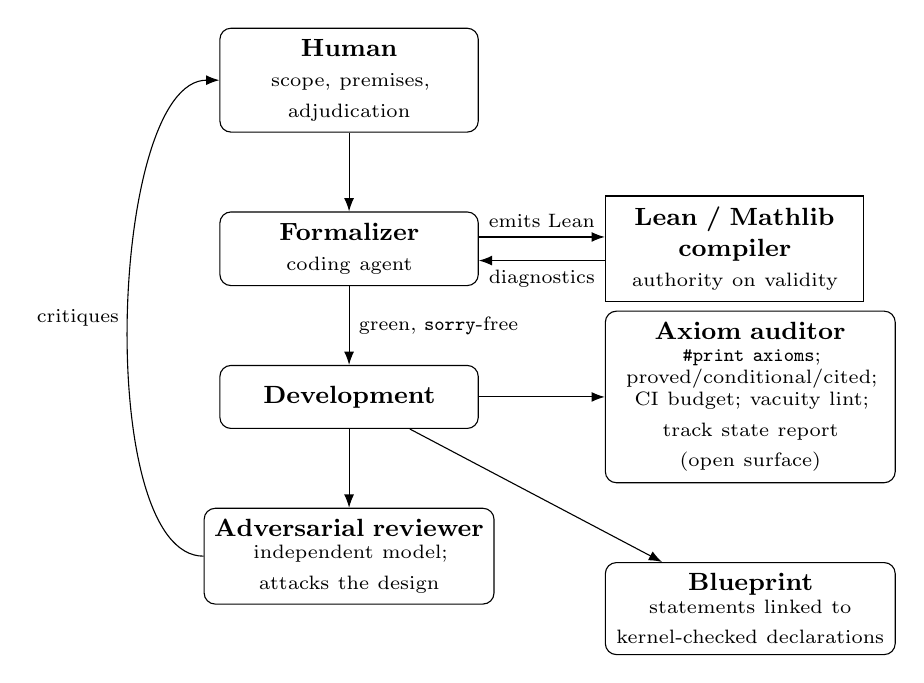
\begin{tikzpicture}[
  >=Latex, node distance=10mm and 16mm,
  box/.style={draw, rounded corners, align=center, inner sep=4pt, font=\small,
              minimum height=8mm, text width=30mm},
  oracle/.style={draw, align=center, inner sep=4pt, font=\small,
                 minimum height=8mm, text width=30mm},
  lbl/.style={font=\scriptsize, midway}
]
\node[box] (human) {\textbf{Human}\\\scriptsize scope, premises, adjudication};
\node[box, below=of human] (form) {\textbf{Formalizer}\\\scriptsize coding agent};
\node[oracle, right=of form] (comp) {\textbf{Lean / Mathlib}\\\textbf{compiler}\\\scriptsize authority on validity};
\node[box, below=of form] (dev) {\textbf{Development}};
\node[box, right=of dev, text width=34mm] (aud) {\textbf{Axiom auditor}\\\scriptsize \texttt{\#print axioms};\\proved/conditional/cited;\\CI budget; vacuity lint;\\track state report (open surface)};
\node[box, below=of dev, text width=34mm] (rev) {\textbf{Adversarial reviewer}\\\scriptsize independent model;\\attacks the design};
\node[box, below=of aud, text width=34mm] (bp) {\textbf{Blueprint}\\\scriptsize statements linked to\\kernel-checked declarations};

\draw[->] (human) -- (form) node[lbl,right]{};
\draw[->, transform canvas={yshift=1.5mm}] (form) -- (comp) node[lbl,above]{\scriptsize emits Lean};
\draw[<-, transform canvas={yshift=-1.5mm}] (form) -- (comp) node[lbl,below]{\scriptsize diagnostics};
\draw[->] (form) -- (dev) node[lbl,right]{\scriptsize green, \texttt{sorry}-free};
\draw[->] (dev) -- (aud);
\draw[->] (dev) -- (rev);
\draw[->] (dev) -- (bp);
\draw[->] (rev.west) .. controls +(left:14mm) and +(left:14mm) .. (human.west)
      node[lbl,left,pos=0.5]{\scriptsize critiques};
\end{tikzpicture}
\caption{The closed, audited loop. The compiler is the authority on mechanical correctness; the
reviewer and the axiom audit address conceptual soundness; the human owns scope and premise
control.}
\label{fig:loop}
\end{figure}

\subsection{The formalizer: a coding agent with compiler self-correction}

The formalizer is a general-purpose coding assistant, repurposed so that its output language is
Lean rather than software and its oracle is the Mathlib build rather than a test suite. In practice
this is a tight inner loop. The agent proposes a definition or a proof term, invokes the build,
reads the diagnostics (an unsolved goal, a type mismatch, an unknown identifier, a failed tactic),
and revises, iterating until the kernel accepts the increment. The diagnostics are unusually
informative compared with a failing software test, because Lean reports the exact remaining goal
state, which functions as a precise specification of what is still to be proved, so the agent's
search is guided rather than blind. Two disciplines make this reliable. The first is to ship green
increments: each unit of work ends with a compiling, \texttt{sorry}-free addition, committed to version
control only when the kernel accepts it, so the development never carries an unproved gap labelled
as proved. The second is to allow no silent \texttt{sorry}: the placeholder that lets Lean accept an
unproved statement is treated as a build failure by policy, not a convenience, so the agent cannot
make progress by deferring a hard step. Mechanical correctness is therefore continuous and
non-negotiable, and it is delegated entirely to the compiler. The agent is never the authority on
whether a proof is valid.

What the formalizer is not good at is what the rest of the loop supplies. Faced with a hard lemma
it cannot close, the agent's path of least resistance is to introduce an \texttt{axiom}, a declaration the
kernel accepts without proof, and to proceed. This is legitimate as a temporary interface, but it
is also where unsoundness enters, because the agent has little incentive, and limited ability, to
notice that the axiom it wrote is false, vacuous, or assumes the very thing downstream theorems
will "prove." The audit (§3.5) makes every such axiom visible, and the reviewer (§3.3) attacks it.

\subsection{The adversarial reviewer: an independent model critiquing design}

Compiler-checking guarantees that a proof is valid. It is silent on whether the statement is the
intended one, whether a convenient axiom smuggles in the conclusion, and whether the surrounding
prose claims more than the Lean delivers. These are conceptual judgments, and a single agent is
poor at them about its own work, because the commitments that produced a design are the same
commitments that hide its flaws from the inside, and an agent that has just spent effort making a
module compile is inclined to regard it as finished. We therefore assign conceptual review to a
different model (GPT-5.5-Pro) with a different training lineage, invoked after each significant step
rather than only at the end, so that a flawed design is caught before downstream work is built on
it.

The reviewer's prompt is adversarial. It is asked to find hypotheses that are vacuous or trivially
satisfiable, meaning an antecedent that constrains nothing; to find axioms that are over-strong or
simply false, and to attempt an explicit counterexample; to find circular dependencies, where a
result is used, directly or transitively, in establishing one of its own premises; and to find
places where the natural-language statement of a theorem, or the paper's description of it,
overclaims relative to the formal content. The reviewer is not asked to check proof validity. That
is the compiler's job, and asking a language model to do it would reintroduce the unreliability the
proof assistant removes. Its remit is narrowed to the soundness questions the compiler cannot
answer. Its critiques are advisory rather than authoritative: the human adjudicates, and the
reviewer is sometimes wrong in both directions (§5.2). But it is independent, and independence of
vantage, the property the LLM-as-judge literature identifies as the source of value \cite{r19,r22},
surfaces the failure modes the formalizer cannot see in itself. Section 4.4 documents two cases in
which this independence was decisive.

\subsection{Human direction: scope, adjudication, premise control}

The human is not eliminated, and the paper does not pretend otherwise. The contribution is a
division of labour that concentrates scarce human judgment, not a claim of autonomy. Three
responsibilities are irreducibly human in our setup. The first is scope: choosing which results to
attempt and in what order, including the strategic decision of which conjectures are worth the cost
of formalization and which are better left as cited frontier. The second is premise control:
deciding which assumptions may enter as a named axiom, and which must be proved outright or recast
as an explicit hypothesis on the theorems that use them. This is the most consequential lever over
soundness, because it determines what the audit will later expose and what the budget will count;
converting a tempting axiom into an explicit hypothesis is the standard way a hidden assumption is
brought into the open, and it reappears in §4.5, Case 2. The third is adjudication: resolving
disagreements between the formalizer and the reviewer, deciding when a critique warrants a redesign
rather than a clarification, and ruling on whether a proposed statement faithfully captures the
intended claim. The value of the method is that it routes the two models' output through these
decisive human decisions while delegating mechanical proof search to the formalizer and
first-pass conceptual critique to the reviewer, so the human spends attention on premises and
adjudication rather than on proof bookkeeping.

\subsection{Soundness instrumentation: the axiom budget and proved/conditional/cited audit}

The audit is central to the trust claim, and it works because modern proof assistants expose their
own trusted base. In Lean, the command \texttt{\#print axioms F} reports the exact set of axioms that the
term \texttt{F} transitively depends on, computed by the kernel rather than by inspection of the source,
so nothing a proof uses can escape it. We maintain a dedicated audit module containing such a
directive for every top-level theorem (830 of them in the case study), and we classify each
dependency into three buckets. A result is proved when its axiom set contains only the standard
logical axioms of the system, which for Lean are \texttt{propext}, \texttt{Classical.choice}, and \texttt{Quot.sound},
the axioms that every ordinary theorem in the library uses and that we do not count against the
project. It is conditional when it additionally depends on a named domain assumption that the
project introduced as an \texttt{axiom}; each such assumption is listed, with a statement of what it
asserts and why it is not yet proved. It is cited when the surrounding argument appeals to an
external result that is not formalized here at all, such as a continuum theorem available only in
the literature. The project-specific axioms, the conditional bucket, are counted into a single
budget.

Two policies turn this from a report into an instrument. First, a continuous-integration guard
fails the build if the count of project-specific axioms rises without an accompanying written
justification, so the budget can only ratchet down over time; an analyst who wants to add an
assumption must say so, on the record. Second, a companion document narrates the discharge of each
axiom, recording what it asserted and the theorem or construction that replaced it, so the audit is
a verifiable history rather than only a number. The boundary between what is established and what is
assumed is thereby made machine-checked and public, and its movement becomes an observable
quantity. When that boundary's project-axiom count reaches zero, the statement "the deductive core
rests on no assumption beyond standard logic" is not a claim to be trusted but a CI result anyone
can reproduce.

One subtlety, which §4.5 shows is not hypothetical, is that the axiom count is blind to a vacuous
or inconsistent axiom. A declared assumption whose hypothesis is trivially true contributes one to
the count while constraining nothing, and removing it lowers the count without improving soundness;
the inconsistency it introduced was the real problem. The budget therefore needs a companion that
inspects axiom content, not only cardinality, a point we return to in §3.7 and §4.5.

The axiom budget governs assumptions declared as \texttt{axiom}, but a result can also rest on
assumptions carried as ordinary \emph{hypotheses} on its statement; an honest audit must make that
surface visible too, since a hypothesis is just an axiom local to one theorem. We therefore run two
further instruments over the top-level theorems, both of them scripts that anyone can re-execute. The
first is a hypothesis ledger: for each target it separates the data binders (the objects a theorem
speaks about) from its propositional hypotheses, and buckets the latter into physical inputs,
kinematic setup, and regularity or background conditions, so the genuine physical-assumption surface
is legible at a glance rather than buried among smoothness side-conditions. The second is a
redundancy probe: for each hypothesis it removes the binder and asks whether a heuristic tactic can
re-derive it from the remaining binders and the library; if so, the hypothesis was redundant and is
flagged for internalization, tightening the statement. The probe is deliberately one-directional. A
hypothesis it closes is genuinely removable, but one it leaves standing is only *not closed by
the heuristics tried*, which does not prove the hypothesis irreducible; the instrument is a lower
bound on redundancy, not a certificate of minimality, and we report it as such. Together with the
axiom budget and the vacuity lint, these give a four-part picture of what a result assumes: which
axioms it invokes, whether any are vacuous, which hypotheses it carries, and which of those are
redundant.

These per-result checks are aggregated, finally, into a goal-directed \emph{state report} for a \emph{track},
a target theorem together with the spine of lemmas that reaches it. The report is driven by a small
version-controlled manifest naming the track's theorems, the axioms it is permitted to use, and the
curation rules that sort hypotheses into physical, setup, and regularity piles; from that manifest it
is regenerated deterministically. For the track's capstone it lists the axioms each result actually
depends on, the complete hypothesis surface, including assumptions *packed inside data-structure
arguments*, which a naive binder count silently misses, the redundancy-probe verdict, and a
partition of the surface into proved, conditional, and open. Every line carries a provenance badge
separating a kernel fact from a prober verdict from a human curation label from our own
interpretation, so the report can neither upgrade "not discharged by the probe" into "mathematically
necessary" nor pass an editorial label off as a Lean fact. Its purpose is direction, not
record-keeping: the open and physical piles are, literally, the assumptions still to discharge, and a
diff between two runs reports exactly which axioms were retired and which hypotheses were closed since
the last. This is what makes the loop goal-directed rather than merely green; after each increment
the human and the formalizer read the remaining open surface and choose the next assumption to
internalize or prove, and the budget's descent toward zero is that open pile emptying out.

\subsection{The link-checked blueprint bridge}

An AI-formalized theory that only Lean experts can read fails the people who must evaluate it, here
physicists, who will not and should not be asked to audit proof terms. We therefore maintain a
blueprint: a document of ordinary mathematical statements in which each statement is annotated with
the name of the Lean declaration that proves it. A checker, run in continuous integration, verifies
that every such name resolves to a real, kernel-checked declaration in the build, so the
human-readable exposition cannot silently drift from the formal development; if a referenced
declaration is renamed or removed, the check fails. A dependency graph renders the logical structure
of the development, with each node coloured according to whether its statement, and its proof, are
formalized, so a reader sees at a glance which parts of the narrative are backed by the kernel and
which are still prose.

Earlier tools generate blueprints as a one-off export \cite{r31,r44}; the artifact here is instead an
integral, continuously-link-checked bridge. A formalized tag in the human-readable document resolves
to a declaration the kernel accepts, and the link is maintained in CI alongside the build and the
audit. We are careful about what this guarantees and what it does not: the checker verifies that
every tag \emph{resolves to a real, kernel-checked declaration}, it prevents dangling references and
silent drift when a declaration is renamed or removed, but it does \textbf{not} verify that the prose
\emph{faithfully paraphrases} the theorem it points to. Name resolution is not semantic equivalence;
catching a prose statement that overclaims relative to its Lean target remains a job for human
reading and the adversarial reviewer. Within that limit, the bridge lets a domain expert read the
mathematics in their own language and click any formalized claim down to the exact declaration that
backs it, which is a concrete partial answer to the objection that AI-generated technical content
cannot be trusted.

\subsection{Protocol and reproducibility}

A round of the loop runs as follows. First, the human fixes a target result and the set of premises
that may be assumed for it. Second, the formalizer produces a compiling, \texttt{sorry}-free increment,
iterating against the compiler as in §3.2. Third, the axiom auditor records the increment's axiom
dependencies via \texttt{\#print axioms} and updates the budget, and a vacuity lint scans the new code for
syntactically vacuous propositional bodies, definitions or conclusions that are literally \texttt{True}
(\texttt{:= True}, \texttt{→ True}, \texttt{∀…, True}), complementing the count with a check on axiom content. Fourth, the adversarial reviewer critiques the design along the four axes of §3.3.
Fifth, the human adjudicates, either accepting the increment, ordering a redesign, or converting an
axiom into an explicit hypothesis on the consuming theorems. Role boundaries are fixed and do not
blur: the compiler is the sole authority on proof validity; the reviewer never edits proofs and
never has the last word; the human alone admits an axiom into the budget. Each round then closes by
regenerating the track's state report (§3.5); its open pile sets the next round's target and its
run-to-run diff records what was discharged, so successive rounds are steered by what remains to be
proved rather than by what already compiles.

Reproducibility of the \emph{artifact} is built in rather than asserted, and we give the specifics. The
full development, the per-theorem audit module, the budget-check and vacuity-lint scripts, the
track-state tool and its track manifests, and the blueprint are public at
\texttt{github.com/kaplan196883/QIQT-H}, commit \texttt{83dc08e}, built with the Lean toolchain
\texttt{leanprover/lean4:v4.30.0} (the pinned Mathlib revision is the one vendored in the repository).
Every metric in §4 is regenerated from source: \texttt{lake build QIQTH} reproduces the green, \texttt{sorry}-free
build; \texttt{scripts/axiom\_budget\_check.sh} reproduces the project-axiom count of zero; the vacuity lint
is a script; the per-result axiom and hypothesis surface (Appendix A) is regenerated by
\texttt{python scripts/lean-track.py report -c tracks/gr.toml}, which calls Lean's \texttt{collectAxioms} directly;
and the blueprint's claim-to-proof links are checked by the bundled checker. The "roughly 2,010"
theorem count is an approximate lemma tally; the exact, audit-relevant numbers (192 modules, 830
\texttt{\#print axioms} directives, 0 project axioms, 0 \texttt{sorry}, 1 benign vacuity site) are exact and
script-reproducible. We regard this property, that the paper's quantitative soundness claims can be
re-derived from the artifact rather than taken on faith, as part of the methodology rather than an
afterthought. We are explicit, by contrast, about what is \emph{not} reproducible: the formalizer and
reviewer are proprietary models, and we do not claim a replayable transcript of the loop, the
checkable object is the audited final artifact, not the agent trajectory (§5.3).

\subsection{Process metrics and an instrument ablation}

A methodology paper should say what running the loop cost and whether its parts pull their weight. We
report both, and are candid about what we did and did not measure. Two honesty boundaries up front:
the formalizer's individual calls were not logged, so commit counts are a \emph{lower-bound proxy} for
iterations, not a true call count; and the figures below are a single-team, single-toolchain case
study, regenerated from git by \texttt{scripts/process\_metrics.sh}.

\begin{table}[ht]
\centering
\caption{Process metrics (regenerated from git at the pinned commit).}
\begin{tabularx}{\linewidth}{@{}>{\raggedright\arraybackslash}p{0.60\linewidth}Y@{}}
\toprule
\textbf{Quantity} & \textbf{Value} \\
\midrule
Active span & \textasciitilde{}30 days (2026-05-25 → 2026-06-24) \\
Commits (total / touching \texttt{lean/}) & 1,455 / 1,016 \\
Commits referencing the reviewer (GPT-5.5) & 61 \\
Commits referencing an axiom or its discharge & 231 \\
Project-axiom trajectory & 57 → 40 → 37 → 35 → 33 → 32 → 31 → 29 → 21 → 17 → 8 → 7 → 6 → 0 (13 events) \\
Adversarial-review rounds (this paper) & 3 (reject → borderline → accept) \\
Reviewer saves, kernel-checked & 2 (a false axiom; an inconsistent one) \\
\bottomrule
\end{tabularx}
\end{table}

The trajectory is the load-bearing process metric: a continuously audited, CI-enforced descent to
zero project axioms, non-monotone because several passes \emph{introduced} a named interface axiom to make
a new conditional result explicit before discharging it; the budget rising is the audit working, not
failing.

Whether the loop's \emph{components} earn their place is the harder question, and the honest answer needs
a comparison, not a narrative. We ran a small \textbf{instrument ablation}: a controlled set of seven Lean
declarations, five seeded faults spanning the failure taxonomy (a false-but-well-typed axiom; an
inconsistent \texttt{True}-antecedent axiom; a circular/over-strong hypothesis; a vacuous \texttt{:= True}
predicate; a \texttt{sorry}) and two sound controls (a clearly-labelled interface axiom; an ordinary proved
lemma), run past each instrument. The deterministic instruments are scored against their exact
specification (verified by running each script's logic); the reviewer is a single \emph{blind}
GPT-5.5-Pro pass, the seven declarations carry neutral names (e.g. \texttt{gleason\_naive},
\texttt{locality\_from\_dilation}), are presented in fixed order, and the reviewer is asked only to classify
each as sound or unsound, \emph{not} told how many faults the set contains. The fault set, the exact
prompt, and the verbatim verdicts are archived with the artifact. We distinguish \emph{surfacing} (an
instrument flagging that something needs human attention, e.g. the budget disclosing that an axiom
was added) from \emph{diagnosis} (identifying the fault as unsound): the structural instruments only
surface, whereas the reviewer diagnoses.

\begin{table}[ht]
\centering
\caption{Instrument ablation: which of 5 seeded faults each configuration surfaces vs. diagnoses (with false positives on 2 sound controls).}
\begin{tabularx}{\linewidth}{@{}YYYYY@{}}
\toprule
\textbf{Configuration} & \textbf{Faults flagged (of 5)} & \textbf{False axiom diagnosed} & \textbf{Over-strong hyp. diagnosed} & \textbf{Sound controls misflagged} \\
\midrule
Compiler (green build) & 0/5 (all build; \texttt{sorry} only warns) & no & no & 0/2 \\
+ axiom budget & 4/5 \emph{surfaced}, \texttt{sorry} + the 3 fault-axioms disclosed as \emph{added axioms} (not judged false); misses the over-strong hypothesis (it adds no axiom) & no (surfaced, not diagnosed) & no & 0/2 \\
+ vacuity lint & 1/5 (the \texttt{:= True} predicate; a \texttt{(h : True)} binder is not matched) & no & no & 0/2 \\
+ independent reviewer (blind) & 5/5 \emph{diagnosed} & \textbf{yes} & \textbf{yes} & \textbf{0/2} \\
\bottomrule
\end{tabularx}
\end{table}

The point is not the headline 5/5 but the \emph{profile}, and the surfaced/diagnosed split is the whole
story. The structural instruments surface structural faults, \texttt{sorry} and added axioms (budget),
\texttt{:= True} bodies (lint), but cannot \emph{diagnose} semantic soundness: a false-but-well-typed axiom is
disclosed by the budget only as "an axiom" (the same signal a \emph{legitimate} labelled assumption
emits, so disclosure is not diagnosis), and a circular/over-strong hypothesis adds no axiom and no
\texttt{sorry}, so it is invisible to all three. Those two faults, exactly the kinds the two historical
reviewer saves (§4.5) belong to, were diagnosed only by the independent reviewer, which also did not
misflag either sound control. This is direct evidence for the division of labour the paper argues:
the compiler owns mechanical correctness, the budget and lint own a \emph{structural} slice of soundness,
and the reviewer covers the \emph{semantic} residue they cannot see.

We hold this evidence to its size. It is one blind pass of one model version over seven hand-designed,
relatively legible faults; it is an indicative profile, not a catch rate, and there is selection bias
toward clear faults, the historical Case 1 (§4.5) took the reviewer \emph{three} passes, so the perfect
single-pass score here should not be read as reliability on subtle faults. A larger pre-registered,
multi-model study is future work (§5.3). The deterministic cells are determinate and reproducible; the
reviewer cell is stochastic and version-specific. The fault set and verdicts are archived with the
artifact.

\section{Case Study: From a Finite-Information Bound to the Einstein Field Equations}

The target framework, QIQT-H, is a foundations-of-physics proposal that we treat strictly as a
formalization target, not as a claim to defend. Its single organizing premise (a finite-information,
Bekenstein-type capacity bound on bounded spacetime regions) reaches in two directions: down to the
quantum measurement problem, and out to gravity. We describe it neutrally, then report the
central theorem the loop produced for this case study (a machine-checked, project-axiom-free,
conditional derivation of the Einstein field equations),
the rest of the development, and what is and is not established. The point of the case study is to
stress the loop and its instruments on a demanding, contested, non-benchmark target, not to argue
for the physics.

\subsection{The target theory, in neutral terms}

QIQT-H is a single-world, exactly-unitary framework whose one physical input is that the physical
instantiation of a state in a bounded spacetime region carries only finite information, bounded by a
holographic (Bekenstein-type) capacity \cite{r40}. On the measurement side this is argued to make
multi-record macroscopic states non-instantiable, so a single definite record obtains per run, with
a non-dynamical actuality selector fixing which record and the Born rule appearing as an across-run
frequency \cite{r32,r33,r34}; the proposal continues a finite-information line of approaches to
measurement \cite{r41}. On the gravitational side the same capacity bound plays the role of the
area-entropy relation in a thermodynamic, Jacobson-style route to the field equations \cite{r46}. It
is set out in a companion paper \cite{r42}, and the Lean development we report on is public
\cite{r43}. Whether these physical claims are true is not our subject; our subject is whether the
framework's deductive core can be formalized end to end, honestly audited, and rendered legible. The
framework's own authors flag its central physical postulates as open, and the formalization respects
that boundary exactly.

\subsection{The case-study theorem: the Einstein field equations from a finite-information bound}

The case study's central theorem, \texttt{QIQTH.QiqtToGR.qiqt\_bekenstein\_gives\_gr}, is a single
end-to-end Lean statement whose conclusion is the Einstein field equations: there exists a constant
$\Lambda$ such that, at every point and for all indices, $a\,T_{\mu\nu}=G_{\mu\nu}+\Lambda\,g_{\mu\nu}$,
where $G$ is the Einstein tensor assembled from the metric by the standard Christoffel/Ricci
construction over a smooth coordinate domain (\texttt{QIQTH.Curvature}; the exact Lean definitions of the
metric, connection, Ricci and Einstein tensors, and the full theorem signature are in Appendix A).
It is project-axiom-free (it uses only Lean's standard axioms) and \texttt{sorry}-free,
and it follows the thermodynamic, equation-of-state route to gravity pioneered by Jacobson \cite{r46},
in which the Einstein equations arise from a local Clausius relation $\delta Q=T\,\delta S$ on local
causal horizons, with the temperature the local Unruh temperature \cite{r48} and entropy proportional
to horizon area.

What makes this a genuine \emph{derivation from the framework}, rather than an assumption of the area
law, is that QIQT-H's own content supplies the thermodynamic input as theorems. Along each local null
generator, the finite-information capacity \emph{bound} $S\le\eta A$ (the Bekenstein-type content,
Lean \texttt{shannon\_le\_log\_card}), its saturation at the reference, and relative-entropy positivity
(Klein's inequality) together \emph{derive} the differential first law $\delta\langle K\rangle=\eta\,\delta A$
(\texttt{differential\_area\_law}); no hypothesis asserts the area law or the conclusion. Two
physics facts that Mathlib cannot prove are then introduced as \emph{explicit, labelled hypotheses}
(never Lean axioms): the Bisognano-Wichmann identification of the wedge-modular flow with the boost,
which supplies the heat flux $\delta\langle K\rangle=(2\pi/\hbar)\,T_{kk}$ \cite{r47}, and Raychaudhuri
focusing, which supplies the area rate $\dot{A}=R_{kk}$ \cite{r49} (the latter itself reduced, via a
machine-checked Raychaudhuri equation, to a single area-versus-expansion modelling identification).
These yield Jacobson's pointwise per-null premise; a machine-checked lemma then turns a symmetric
tensor that vanishes on the entire null cone into a scalar multiple of the metric, and conservation
plus the contracted Bianchi identity fix the integration constant as a genuine cosmological constant.

All of the differential geometry is machine-checked and project-axiom-free: the second Bianchi
identity, the contracted-Bianchi conservation law $\nabla^\mu G_{\mu\nu}=0$ (divergence-freeness of the Einstein
tensor), metric compatibility, the trace identities, the null-cone-to-tensor step for a general
Lorentzian metric, and the constancy of $\Lambda$. Table 3 sorts the chain into what
QIQT-H derives, what is cited, and what is machine-checked geometry.

\begin{table}[ht]
\centering
\caption{The QIQT-H + Bekenstein ⇒ Einstein-field-equations chain, by status.}
\begin{tabularx}{\linewidth}{@{}>{\raggedright\arraybackslash}p{0.60\linewidth}Y@{}}
\toprule
\textbf{Step} & \textbf{Status} \\
\midrule
Capacity bound $S\le\eta A$, saturation, Klein positivity & Derived in QIQT-H (theorems) \\
Differential first law $\delta\langle K\rangle=\eta\,\delta A$ & Derived from the above \\
Wedge-modular $=$ boost heat flux $T_{kk}$ (Bisognano-Wichmann) & Cited (explicit hypothesis) \\
Raychaudhuri focusing $\dot{A}=R_{kk}$ & Cited hypothesis; geometric core machine-checked \\
Null-cone→tensor, 2nd/contracted Bianchi, $\nabla^\mu G_{\mu\nu}=0$, constant $\Lambda$ & Machine-checked, project-axiom-free \\
Einstein field equations $a\,T_{\mu\nu}=G_{\mu\nu}+\Lambda g_{\mu\nu}$ & Machine-checked conclusion \\
\bottomrule
\end{tabularx}
\end{table}

The honest scope is therefore precise, and we state it in both directions. The formalization certifies
that, \emph{conditional on} the two cited physics facts and the standard structural inputs (a
Lorentzian congruence, $\nabla^\mu(aT)=0$, regularity of the scalar $f$, per-generator
differentiability), QIQT-H's capacity bound and Klein positivity \emph{derive} the Einstein field
equations, and that this derivation rests on no hidden axiom. It does \emph{not} establish the cited
inputs themselves: Bisognano-Wichmann and Raychaudhuri are genuine theorems of algebraic QFT and
Lorentzian geometry, but here they are assumed; nor does it establish the framework's physical
capacity postulate. An in-progress effort formalizes the one-particle Bisognano-Wichmann property
directly, which would move the modular-flux input from cited toward derived for the free field.

This scope statement is not editorial: it is read off the theorem by the hypothesis-audit scripts of
§3.5, which anyone can re-run. The ledger reports that \texttt{qiqt\_bekenstein\_gives\_gr} takes 14
data binders and 23 propositional hypotheses, and buckets the hypotheses as four physical inputs (the
Clausius/area-saturation floor), one Raychaudhuri-focusing input, one wedge-modular boost-flux input,
one stress-energy conservation condition, three per-generator differentiability conditions, and
thirteen regularity or background conditions (metric symmetry and smoothness, the frame, and the
constants). The genuine physical-assumption surface is thus exactly the three inputs the prose names;
everything else is kinematic setup or regularity. Running the redundancy probe over the case-study
theorem and the eight related capstones of the chain returns zero auto-dischargeable hypotheses: no
labelled input is closed by the heuristic tactics, so the surface is not padded with hypotheses the
library could already supply. Consistent with §3.5, this is a lower bound on minimality rather than a
proof of it, but it shows the assumption surface is tight under an automated check, and it makes the
premise ledger of the case-study theorem a reproducible artifact rather than a narrative claim.

Two limits of this evidence must be stated plainly, because the audit is easy to over-read. First,
project-axiom-freedom is not assumption-freedom: a theorem carrying 23 labelled hypotheses rests on
those hypotheses exactly as if they were local axioms, which is why we list them in full (Appendix A)
rather than only counting them. Second, and more subtly, neither the zero project-axiom count nor the
zero-auto-dischargeable verdict establishes that the 23 hypotheses are \emph{jointly satisfiable}: a
project-axiom-free theorem whose premises were secretly contradictory would be vacuously true, and
the syntactic vacuity lint of §3.5 need not catch it. The audit certifies the absence of project
axioms, not the consistency of the premise set. The rigorous remedy is a \emph{model}, an explicit
instantiation of every binder under which all 23 hypotheses simultaneously hold.
We supply such a witness, machine-checked: a flat (Minkowski) background with vanishing
stress-energy, \texttt{g = gi = (fun \_ => gm)} (the constant reference metric, with $gm\cdot gm = I$), the
identity frame, $T=0$, and zero entropy/modular-energy/area. The Lean theorem
\texttt{qiqt\_bekenstein\_gives\_gr\_satisfiable} (Appendix A) discharges all 23 hypotheses under this model and
\emph{applies} the case-study theorem, obtaining its conclusion, the true vacuum equation $G_{\mu\nu}=0$.
The one non-trivial lemma is that the Ricci tensor of a constant metric vanishes (its Christoffel
symbols are built from metric derivatives, which are zero); we prove it, and the witness is itself
project-axiom-free (\texttt{\#print axioms} returns only the three standard axioms). So the case-study's
premise set is demonstrably consistent and the theorem non-vacuous \emph{in the logical sense}: its hypotheses
are jointly satisfiable, ruling out the failure mode where the result holds only by explosion. We are
equally clear about what the witness does \emph{not} show: the model is deliberately degenerate (flat,
$T=0$), so the flux, focusing, area-law, and conservation premises all reduce to $0=0$ and the
conclusion to the vacuum equation. It exhibits a model of the premise set; it does not exercise the
derivation on a curved or matter-bearing instance, and "non-vacuous" should be read throughout as
"jointly satisfiable," not "physically rich." We also keep the general distinction explicit: the
audit shows no project axiom and no syntactically vacuous premise, which for an \emph{arbitrary} theorem
is weaker than a consistency proof, and making such a witness routine is methodological future work
(§5.3); but for the case-study theorem the satisfiability is now machine-checked.

\subsection{The rest of the development, with artifact metrics}

Beyond the case-study theorem, the development formalizes the framework's other layers, whose epistemic
shapes differ and which the method's audit keeps explicit. A
first layer mechanizes the no-collapse mechanism. From a finite additive capacity and a
redundant-record (Spectrum Broadcast) structure \cite{r45}, it derives that at most one macroscopic record can
be co-instantiated, with the capacity threshold itself derived from orthonormality rather than
stipulated, and a per-collision distinguishability derived from a textbook interaction Hamiltonian.
A second layer treats the Born rule as a conditional representation theorem. An effect-Gleason
argument \cite{r35,r36} shows that a positive, normalized, non-contextual outcome assignment must be the Born
functional, and a join assembles unique actual histories carrying the Born product law under
explicit product-preparation and non-contextuality hypotheses. This layer is accompanied by a
deliberate suite of negative results: that linear unitary decoherence does not concentrate branch
weights, that the structural axioms do not single out Born among distributions, that support
preservation is strictly weaker than Born equivariance \cite{r37}, and that operational click-statistics
underdetermine the underlying measure. Together these establish that the conditional theorem's
premises are necessary rather than decorative. A third layer lifts the finite marginals to a
covariant, sigma-additive typicality measure over global measurement histories via a
Kolmogorov-style extension, state-agnostically, with an operational no-signaling result for
arbitrary entangled states. A fourth layer discharges the abstract normal-state input with a
genuine normal state on the algebra of bounded operators and exhibits a free-field, boost-invariant
instance. Above these sits a continuum tower, comprising bounded spectral theory and
projection-valued measures, Fock space and Weyl/CCR structure, and the entropy and data-processing
machinery; it is under construction toward the framework's open problems and is not yet complete.

Naming the layers matters because the audit treats them uniformly. Every theorem above, across all
four layers and the in-progress tower, is subject to the same \texttt{\#print axioms} discipline, and every
one of them, including the negative audits, which are themselves theorems that something does not
follow, lands in the proved bucket.

The artifact is quantified rather than asserted. As of 2026-06-21 the development comprises \textbf{192
modules and approximately 2,010 theorems and lemmas}, with \textbf{830 \texttt{\#print axioms} directives} in a
dedicated audit module. It builds green, contains \textbf{no \texttt{sorry}}, and depends on \textbf{zero
project-specific axioms}, so every audited theorem rests only on the three standard Lean axioms. A
vacuity scan (§4.5) reports a single benign site. Table 4 summarizes.

\begin{table}[ht]
\centering
\caption{Artifact metrics (verified 2026-06-21).}
\begin{tabularx}{\linewidth}{@{}>{\raggedright\arraybackslash}p{0.60\linewidth}Y@{}}
\toprule
\textbf{Quantity} & \textbf{Value} \\
\midrule
Lean modules & 192 \\
Theorems / lemmas & \textasciitilde{}2,010 \\
\texttt{\#print axioms} directives (audit) & 830 \\
Project-specific axioms & 0 \\
\texttt{sorry} occurrences & 0 \\
Vacuity-lint sites & 1 (benign; an indiscrete-preorder definition) \\
Build status & green \\
\bottomrule
\end{tabularx}
\end{table}

\subsection{The audit in action: the ratchet, and the honesty boundary}

The audit's signal is a trajectory rather than a single number. Over the project's life the count of
project-specific axioms fell

\[
57 \to 40 \to 37 \to 35 \to 33 \to 32 \to 31 \to 29 \to 21 \to 17 \to 8 \to 7 \to 6 \to 0.
\]

The ratchet is honest about its own shape. Several passes raised the count, introducing a named
interface axiom to make a new conditional result explicit before later discharging it; the budget
measures exposed assumptions, and exposing one is progress over hiding it inside a proof. The
discharges are not bookkeeping, because each replaced an assumption with mathematics. An eleven-axiom
relative-entropy interface, comprising the abstract properties of Araki relative entropy on which
the framework's entropy arguments depended, including Donald's identity and the Holevo bound
$\chi \le H(p)$, was discharged to theorems by realizing the interface in a finite-dimensional
matrix model and proving the Holevo bound pointwise via operator-monotonicity of the logarithm,
transported through a bridge to C*-matrix structure. An eight-axiom packaging of Donald's identity
was likewise replaced by a typeclass with a concrete, axiom-free instance, as were a four-axiom
data-processing-inequality interface, realized by a concrete mixed-unitary channel, and a
relative-entropy-positivity (Klein) interface. On the Born side, a Goldstein-Struyve "Schur
classification" that had stood as a named axiom was proved outright, as was the attainability half
of the Tsirelson bound by an explicit construction; and the effect-Gleason capstone, that
positivity, normalization, and ray-certainty force the Born functional, was proved, retiring the
false axiom of §4.5. The endpoint is that the deductive core depends on no project-specific axiom
at all: every one of the former interface assumptions is now either a theorem in a concrete
realization or an explicit hypothesis on the theorems that use it.

Three layers must be held apart, and the audit holds them apart (Table 5). The deductive core is
project-axiom-free. The framework's physical postulates, namely the holographic instantiation bound,
the macroscopic-definiteness conjecture, the canonical typicality (Born) principle, and the Lorentz
covariance of the selector, are open, and a project-axiom-free Lean development bears on none of them.
A continuum formalization frontier is in progress. The most important sentence of this section is
therefore the following: a project-axiom-free development in the proof assistant certifies that the
framework's conditional mathematics is correct, given its labelled premises, and rests on no hidden
axiom; it does not establish the physics, and project-axiom-freedom is not consistency of the premise
set (§4.2). We repeat this guard in §5.3.

\begin{table}[ht]
\centering
\caption{The three-layer status boundary.}
\begin{tabularx}{\linewidth}{@{}>{\raggedright\arraybackslash}p{0.60\linewidth}Y@{}}
\toprule
\textbf{Layer} & \textbf{Status (2026-06)} \\
\midrule
Conditional/structural deductive core & Machine-checked, project-axiom-free (standard axioms only) \\
Physical postulates (capacity bound; definiteness; Born; covariance) & Open; not theorems; unaffected by formal discharge \\
Continuum realization (Type II / Fock / modular flow) & Formalization frontier, in progress \\
\bottomrule
\end{tabularx}
\end{table}

\subsection{What the reviewer caught: two soundness saves}

The value of the loop is not that it produced a compiling development, since many systems do that,
but that it produced an audited one, with documented saves the compiler alone would have missed.
Both episodes below are kernel-checked in the published development, so the reader need not take
them on trust.

\textbf{Case 1, a false axiom.} The formalizer initially encoded a Gleason-type step as a named axiom:
that a normalized, additive, homogeneous valuation on quantum effects that is certain on the state's
ray must equal the Born functional. The independent reviewer, on its third pass over the module,
flagged the axiom as false, because it omits positivity. The refutation, which was then itself
formalized, is a two-dimensional weight that satisfies every stated premise yet is not the Born
functional. The false axiom was retired and replaced not by a patch but by proved content: a lemma
deriving ray-support from positivity, and a capstone showing that a positive, normalized,
ray-certain weight is the Born functional. The fix made the result stronger, since Born now follows
from positivity, an honest hypothesis, and it removed an axiom. The lesson is that an independent
vantage catches a capable agent's plausible-but-false premise.

\textbf{Case 2, an inconsistent axiom the counter could not see.} A locality interface was encoded as an
axiom whose hypothesis was the trivially-true proposition. Because a \texttt{True} antecedent constrains
nothing, the axiom in effect asserted a universal equality that is simply false, and any theorem
consuming it inherited an inconsistency. Neither of the habitual checks detects this: the
development builds, and it contains no \texttt{sorry}, yet it rested on a contradiction. The axiom was
removed, and the affected theorem now takes locality as an explicit hypothesis, relocating the
assumption into the open. In response, the project added a third soundness instrument, a vacuity
lint that scans for \emph{syntactically} vacuous propositional bodies, definitions or conclusions that
are literally \texttt{True} (\texttt{:= True}, \texttt{→ True}, \texttt{∀…, True}). It is a syntactic complement, not a
replacement for the reviewer: a vacuity hidden in a \texttt{(h : True)} binder, as in this very case, is
\emph{not} matched by the lint; it is surfaced by the budget (as an added axiom) and diagnosed by the
reviewer, the division of labour the ablation of §3.8 quantifies. The lint currently reports a
single site, which inspection confirms is a legitimate indiscrete-preorder definition rather than a
hidden assumption. This episode captures the paper's
central point: "compiles, no \texttt{sorry}, axiom count zero" is necessary but not sufficient, and
soundness requires auditing for vacuity and inconsistency as well.

We are deliberately modest about what these two episodes prove. They are illustrative, kernel-checked
\emph{existence} cases, concrete demonstrations that an independent reviewer, so positioned, can catch a
false axiom and a vacuous one that a green build and a zero \texttt{sorry} count do not. They are not, by
themselves, a measured catch rate: we did not log every reviewer critique over the project's life,
so we have no project-wide true-positive/false-positive denominator. To put the comparison on a
controlled footing we instead ran the small instrument ablation of §3.8, in which the reviewer caught
both fault families these two saves exemplify, the false-but-well-typed axiom and the
circular/over-strong hypothesis that the structural instruments cannot see, with no false positives
on the sound controls. That ablation is small and indicative rather than definitive (§3.8, §5.3), but
it moves the claim from "the failure mode is real and the instrument can catch it" toward a
reproducible, if modest, detection profile. With that caveat, the loop did not merely yield a green
build; it yielded an audited, shrinking-to-zero conditional base with concrete, checkable saves.

\section{Discussion, Limitations, and Threats to Validity}

\subsection{What generalizes, and how to port it}

The loop and the audit are, by construction, domain-agnostic: nothing in §3 is specific to physics or
to the particular case-study theory. We state this as a \emph{conjecture supported by one case}, not a
demonstrated property, the generality is argued from the structure of the method, and we have not
run it on a second domain or team (§5.3). The construction is a self-correcting formalizer, an
independent adversarial reviewer, a \texttt{\#print axioms}-based proved/conditional/cited audit with a
ratcheting budget, a vacuity lint and a hypothesis ledger over the assumption surface, a goal-directed
track-state report, and a link-checked blueprint. Any formalization effort in which soundness, not
merely compilation, matters could in principle adopt it; whether it pays off elsewhere is exactly
what multi-domain replication would test.

To make the transfer concrete, consider porting the loop to a different domain, say the verification
of a novel cryptographic protocol's security argument, or a new result in distributed-systems
theory. The steps are mechanical. (i) Choose the proof assistant and library that already cover the
most background, whether Lean/Mathlib, Isabelle/HOL, or Coq, so the formalizer spends its effort on
the new content rather than on rebuilding foundations. (ii) Have the human decompose the target into
a deductive core, meaning what should be proved, and a cited frontier, meaning results to assume
from the literature, and fix, per result, which premises may be axioms. (iii) Run the inner
formalize-and-self-correct loop to a green, \texttt{sorry}-free state. (iv) After each module, emit the
axiom audit, classify proved/conditional/cited, and run the vacuity lint. (v) Have an independent
model adversarially review the design for vacuity, over-strong axioms, circularity, and overclaiming.
(vi) Maintain a blueprint linking each human-readable claim to its checked declaration. The only
domain-specific inputs are the target decomposition and the premise policy, both human and both
decisive, and the rest is the same instrument. The pattern is most valuable where the cost of a
hidden assumption is highest: original theories, contested foundations, and safety-relevant or
security-relevant claims, where "it compiles" is the reassurance one must not accept uncritically.
It is least valuable for routine benchmark proving, where the target is externally certified and the
soundness question is already settled.

\subsection{Failure modes and the human's irreducible role}

The method is not autonomous and we do not present it as such, and its failure modes are as
important to report as its successes. The formalizer stalls on genuinely hard lemmas and, often, on
gaps in the underlying library, where a result it needs is simply not in Mathlib and supplying it is
a research task in its own right rather than a matter of search. In such cases the agent's tempting
shortcut is to introduce an axiom, which is why the audit and the reviewer must be running: an
unsupervised formalizer left to clear its own blockers will accumulate assumptions. The reviewer is
sometimes wrong in both directions. It is over-cautious when it flags a sound construction as
suspicious, which is common when a definition is unusual but correct, and over-confident when it
pronounces a module clean that in fact harbours a subtle problem; we observed both. Its value is
therefore statistical and adversarial rather than oracular: it raises candidates, and the human and
the compiler dispose of them. Finally, the human remains the premise gatekeeper, which is the
load-bearing role. The audit makes assumptions visible, but visibility is not acceptability, and a
human still decides which assumptions a result may rest on. The honest claim is that the loop
concentrates scarce human judgment onto premise control and adjudication and removes it from proof
bookkeeping, not that it removes the human.

\subsection{Threats to validity}

Several limits bound the strength of our conclusions. The first is that this is a single case study:
we report one theory, one team, one toolchain, so the method's generality is argued rather than
demonstrated across independent efforts, and multi-team replication is needed. The second is model
and version specificity: the results depend on particular models and their versions, and the
qualitative behaviour, especially the reviewer's catch rate, may shift as models change. The third
is audit completeness: the audit certifies which axioms a result depends on and that none are
vacuous by the lint's criteria, but "no vacuous axiom the lint can see" is weaker than "every
assumption is justified," and a sufficiently subtle mis-formalization of a statement, as opposed to
a proof, remains possible in principle, which is part of why the blueprint bridge and human review
matter. The fourth, and most important, is that the case-study theory's own physics is not closed by
formalization. Driving the deductive core to zero axioms says nothing about whether the holographic
capacity bound, the definiteness conjecture, or the Born principle are physically correct; and the
case-study derivation of the Einstein field equations is explicitly conditional on its two cited inputs
(the Bisognano-Wichmann wedge-modular flux and Raychaudhuri focusing) and standard structural
assumptions, which the formalization records as hypotheses but does not establish. We state this not
as a closing caveat but as a structural feature of what machine verification can and cannot do for
foundational science.

The fifth limit is evidential, and it is now partial rather than total. We report process metrics and
a small controlled instrument ablation (§3.8), which does show that the structural instruments
(compiler, axiom budget, vacuity lint) miss the semantic faults the independent reviewer catches. But
that ablation is small (seven items, one blind pass, one model version), and we still do not report
full quantitative process metrics, true LLM-call counts (commit counts are only a lower-bound proxy),
human hours, project-wide reviewer true-/false-positive rates, or time relative to manual
formalization, nor a large pre-registered multi-model study. The claim is therefore an audited
existence result, a methodology, and an \emph{indicative} ablation, not yet a statistically validated
improvement over a baseline; the larger study is future work. The sixth concerns premise-set consistency: as discussed in §4.2,
project-axiom-freedom certifies the absence of project axioms, not the joint satisfiability of a
theorem's hypotheses. For the case-study theorem we close this with a machine-checked
model witness (the Minkowski/vacuum instantiation of Appendix A), so its premise set is provably
satisfiable; but the methodology does not yet make such a witness \emph{routine} for an arbitrary theorem,
and absent one a contradictory premise set would render a theorem vacuously true without tripping the
syntactic vacuity lint. Finally, the loop
itself is not reproducible: the formalizer and reviewer are proprietary models and we publish no
replayable transcript, so the checkable object is the audited final artifact, not the agent
trajectory.

\section{Conclusion}

AI now produces a great deal of science, and very little of it is machine-checked. We have argued
that the answer is not only to machine-check AI-produced reasoning but to audit its axiom base,
because a proof that compiles can still rest on an assumption that is false, vacuous, or
question-begging, and the two checks practitioners habitually run, "it builds" and "it has no
\texttt{sorry}," cannot tell the difference. We have presented a concrete instrument for closing that gap: a
human-directed loop in which a self-correcting formalizer is paired with an architecturally
independent adversarial reviewer and a continuously maintained, CI-enforced soundness audit, made
goal-directed by a track-state report and exposed through a link-checked blueprint.

As a demanding case study, applied to a new, contested foundations-of-physics framework, the loop
produced a machine-checked,
\emph{project-axiom-free} Lean theorem deriving, \emph{conditionally}, the Einstein field equations
$a\,T_{\mu\nu}=G_{\mu\nu}+\Lambda g_{\mu\nu}$ from the framework's finite-information
(Bekenstein-type) capacity bound by a Jacobson-style equation of state in which the thermodynamic
input is itself derived, while Bisognano-Wichmann wedge-modular flux and Raychaudhuri focusing enter
as explicitly labelled hypotheses and all the differential geometry downstream is machine-checked.
The same project-axiom-free development carries a no-collapse measurement core; in total it
drove the project's axiom count from fifty-seven to zero, with no \texttt{sorry}, across 192 modules
and roughly 2,010 theorems, and it produced two documented, kernel-checkable soundness saves (a false
axiom the reviewer refuted by counterexample, and an inconsistent one the axiom counter could not see,
which motivated a vacuity lint). The contribution is the audited methodology and its instruments, together with this
demonstration on a substantial, non-benchmark development, held throughout under an explicit honesty
boundary: the
formalization certifies that the derivation uses no hidden axiom, given its labelled premises; it
does not, and cannot, establish those cited inputs or the framework's physical postulates, which
remain open, though a machine-checked witness (Appendix A) does establish that the case-study premise
set is jointly satisfiable (via a deliberately degenerate flat/vacuum model), so the theorem is
non-vacuous in the logical sense. We make the strong-sounding negative claim deliberately: this is
not "AI proved general relativity," and the paper's value lies precisely in being able to say exactly
what it is and is not.

Three near-term directions follow. The first is independent multi-team replication, since the
strongest test of a methodology is that others can run it, and the artifact is published so they can.
The second is partial automation of the audit and the reviewer protocol, including richer detection
of vacuity, inconsistency, and circularity than a count and a syntactic lint provide. The third is a
careful study of when the independent reviewer adds value, meaning under what conditions its catch
rate justifies its cost, so that human attention is spent where it is decisive. The broader claim we
wish to defend is modest, and we think it is important for the moment AI-for-science is entering:
AI-assisted formalization is most trustworthy not when it proves the most, but when it is most
honest, and most precisely auditable, about exactly what it has and has not assumed.

\section*{Acknowledgements}

The formalization was carried out with Claude Code (Anthropic) as the formalizer and GPT-5.5-Pro
(OpenAI) as the independent adversarial reviewer, under the author's direction. This AI assistance
is the subject of the paper and is disclosed in full in §3. The development builds on Lean 4 and the
Mathlib library and on the broader interactive-theorem-proving community.

\section{Appendix A: the case-study theorem, its full assumption surface, and axiom audit}

This appendix gives the exact statement of the case-study theorem, the complete list of its labelled
hypotheses, and the kernel's report of the axioms it depends on, so that the claims of §4.2 are
checkable from the text. Everything below is regenerated from the public artifact (§3.7) by
\texttt{python scripts/lean-track.py report -c tracks/gr.toml}, which calls Lean's \texttt{collectAxioms}.

\textbf{Conclusion and data.} \texttt{QIQTH.QiqtToGR.qiqt\_bekenstein\_gives\_gr} takes 14 data binders, a metric
\texttt{g} and inverse \texttt{gi} (each \texttt{Point 4 → Fin 4 → Fin 4 → ℝ}), a stress tensor \texttt{T}, constants \texttt{η hbar a},
a frame \texttt{P}/\texttt{Pinv}, and per-generator entropy/modular-energy/area functions \texttt{S KE A} with derivatives
\texttt{sd kd ad}, and concludes the Einstein field equations:

{\footnotesize\begin{alltt}
∃ Λ, ∀ (x : Curvature.Point 4) (μ ν : Fin 4),
    a * T x μ ν = Curvature.einsteinTensor g gi μ ν x + Λ * g x μ ν
\end{alltt}}

where \texttt{einsteinTensor} is \texttt{ricci − (1/2) scalarCurv · g}, with \texttt{ricci}/\texttt{scalarCurv} built from the
Christoffel symbols of \texttt{g} over the smooth coordinate domain \texttt{Curvature.Point 4} (these definitions
live in \texttt{QIQTH.Curvature}).

\textbf{The 23 labelled hypotheses} (binder name : type), grouped by the curated piles of §3.5:

{\footnotesize\begin{alltt}
-- PHYSICS, genuine inputs (the conditional content); "near 0" = Eventually (nhds 0)
hbound  : ∀ x v, BL (g x) v = 0 → near 0,  S x v t ≤ η * A x v t
hsat    : ∀ x v, BL (g x) v = 0 → S x v 0 = η * A x v 0
hDnn    : ∀ x v, BL (g x) v = 0 → ∀ t, 0 ≤ KE x v t - S x v t
hD0     : ∀ x v, BL (g x) v = 0 → KE x v 0 - S x v 0 = 0
hFlux   : ∀ x v, BL (g x) v = 0 → kd x v = 2*π/hbar * BL (T x) v
hFocus  : ∀ x v, BL (g x) v = 0 → ad x v = BL (fun i j => ricci g gi i j x) v
-- SETUP, per-generator derivative existence
hS : ∀ x v, BL (g x) v = 0 → HasDerivAt (S  x v) (sd x v) 0
hK : ∀ x v, BL (g x) v = 0 → HasDerivAt (KE x v) (kd x v) 0
hA : ∀ x v, BL (g x) v = 0 → HasDerivAt (A  x v) (ad x v) 0
-- CONSISTENCY, stress-energy conservation
conserv : ∀ x ν, Curvature.div02 g gi (fun y a b => a * T y a b) ν x = 0
-- REGULARITY / BACKGROUND, metric, frame, smoothness, constants
hsymm    : ∀ y a b, g  y a b = g  y b a
hsymm_gi : ∀ y a b, gi y a b = gi y b a
hinv     : ∀ y a b, ∑ σ, g y a σ * gi y σ b = (if a = b then 1 else 0)
hCg      : ∀ a b, ContDiff ℝ ⊤ (fun y => g  y a b)
hCgi     : ∀ a b, ContDiff ℝ ⊤ (fun y => gi y a b)
hbar0    : hbar ≠ 0          heta : η ≠ 0          ha : a = 2 * π / (hbar * η)
hT_symm  : ∀ x a b, T x a b = T x b a
hPP      : ∀ x i j, ∑ k, P x i k * Pinv x k j = (if i = j then 1 else 0)
hPP'     : ∀ x i j, ∑ k, Pinv x i k * P x k j = (if i = j then 1 else 0)
hcong    : ∀ x i j, g x i j = ∑ k, ∑ l, P x k i * EinsteinEOS.gm k l * P x l j
hreg     : ∀ f, (∀ y a b, a * T y a b = ricci g gi a b y + f y * g y a b) →
                (∀ x ρ, Curvature.PdiffAt f ρ x)
                  ∧ Differentiable ℝ (fun y => f y + (1/2) * scalarCurv g gi y)
\end{alltt}}

Here \texttt{BL (g x) v} is the bilinear form \texttt{g\_\{ij\} v\textasciicircum{}i v\textasciicircum{}j}, so \texttt{BL (g x) v = 0} is the null condition
selecting horizon generators. The genuine physical surface is the six PHYSICS binders; of these, the
Clausius/area floor (\texttt{hbound}, \texttt{hsat}, \texttt{hDnn}, \texttt{hD0}) is the QIQT-H capacity postulate, and \texttt{hFlux},
\texttt{hFocus} are the cited Bisognano-Wichmann and Raychaudhuri inputs.

\textbf{Axiom audit.} \texttt{\#print axioms QIQTH.QiqtToGR.qiqt\_bekenstein\_gives\_gr} reports

{\footnotesize\begin{alltt}
'QIQTH.QiqtToGR.qiqt_bekenstein_gives_gr' depends on axioms: [propext, Classical.choice, Quot.sound]
\end{alltt}}

These are Lean's three standard axioms and no project-specific axiom (the project-axiom budget is 0). The
redundancy probe of §3.5 returns no auto-dischargeable hypothesis among the 23.

\textbf{Satisfiability witness (machine-checked).} Project-axiom-freedom does not by itself establish that
the 23 hypotheses are jointly satisfiable (§4.2), so we exhibit a model and verify all of them in
Lean. Take \texttt{g = gi = (fun \_ => EinsteinEOS.gm)} (the constant reference metric, with \texttt{gm·gm = I}),
\texttt{P = Pinv = id}, \texttt{T = 0}, and \texttt{S = KE = A = 0} with \texttt{sd = kd = ad = 0}. Then \texttt{hsymm}/\texttt{hinv}/\texttt{hPP}/
\texttt{hcong} hold by computation; \texttt{hbound}/\texttt{hsat}/\texttt{hDnn}/\texttt{hD0} reduce to \texttt{0 ≤ 0} / \texttt{0 = 0};
\texttt{hFlux}/\texttt{hFocus}/\texttt{conserv} reduce to \texttt{0 = 0} once the Ricci tensor of the constant metric is shown to
vanish; \texttt{hreg} forces \texttt{f = 0} (from \texttt{0 = ricci + f·gm} with \texttt{ricci = 0} and \texttt{gm₀₀ = -1}); and the
conclusion holds with \texttt{Λ = 0}, giving the true vacuum equation \texttt{G\_\{μν\} = 0}. The supporting lemma
chain \texttt{christoffel (fun \_ => G) = 0 → riemann = 0 → ricci = 0 → scalarCurv = 0 → einsteinTensor = 0}
(Christoffel symbols of a constant metric vanish, since they are built from metric derivatives) is
proved generically. The witness theorem is

{\footnotesize\begin{alltt}
theorem qiqt_bekenstein_gives_gr_satisfiable :
    ∃ Λ, ∀ x μ ν, (2*π) * 0 = einsteinTensor gW gW μ ν x + Λ * gW x μ ν :=
  QIQTH.QiqtToGR.qiqt_bekenstein_gives_gr gW gW … -- all 23 hypotheses discharged
\end{alltt}}

and \texttt{\#print axioms QIQTH.QiqtGrWitness.qiqt\_bekenstein\_gives\_gr\_satisfiable} returns
\texttt{[propext, Classical.choice, Quot.sound]}, i.e. project-axiom-free. Hence the case-study premise set is
provably consistent and the theorem non-vacuous in the logical (joint-satisfiability) sense. The
model is deliberately degenerate (flat, $T=0$, so flux/focusing/area-law premises reduce to $0=0$
and the conclusion to $G_{\mu\nu}=0$), so it certifies consistency, not a physically rich instance.


\begin{thebibliography}{99}

\bibitem{r1} Lu, C., et al. (2024). \emph{The AI Scientist: Towards Fully Automated Open-Ended Scientific Discovery.} arXiv:2408.06292.
\bibitem{r2} Yamada, Y., et al. (2025). \emph{The AI Scientist-v2: Workshop-Level Automated Scientific Discovery via Agentic Tree Search.} arXiv:2504.08066.
\bibitem{r3} Gottweis, J., et al. (2025). \emph{Towards an AI Co-Scientist.} arXiv:2502.18864.
\bibitem{r4} Brenner, M. P., Cohen-Addad, V., \& Woodruff, D. (2026). \emph{Solving an Open Problem in Theoretical Physics using AI-Assisted Discovery.} arXiv:2603.04735.
\bibitem{r5} Liu, M., \& Fang, J. (2025). \emph{Enhancing Mathematical Reasoning in Large Language Models with Self-Consistency-Based Hallucination Detection.} arXiv:2504.09440.
\bibitem{r6} \emph{The Need for Verification in AI-Driven Scientific Discovery} (2025). arXiv:2509.01398.
\bibitem{r7} \emph{Why LLMs Aren't Scientists Yet: Lessons from Four Autonomous Research Attempts} (2026). arXiv:2601.03315.
\bibitem{r8} Wu, Y., Jiang, A. Q., et al. (2022). \emph{Autoformalization with Large Language Models.} arXiv:2205.12615.
\bibitem{r9} Jiang, A. Q., Welleck, S., et al. (2022). \emph{Draft, Sketch, and Prove: Guiding Formal Theorem Provers with Informal Proofs.} arXiv:2210.12283.
\bibitem{r10} Weng, K., et al. (2025). \emph{Autoformalization in the Era of Large Language Models: A Survey.} arXiv:2505.23486.
\bibitem{r11} Yang, K., et al. (2024). \emph{Formal Mathematical Reasoning: A New Frontier in AI.} arXiv:2412.16075.
\bibitem{r12} Breen, B., Del Tredici, M., et al. (2025). \emph{Ax-Prover: A Deep Reasoning Agentic Framework for Theorem Proving in Mathematics and Quantum Physics.} arXiv:2510.12787.
\bibitem{r13} \emph{LeanMarathon: Toward Reliable AI Co-Mathematicians through Long-Horizon Lean Autoformalization} (2026). arXiv:2606.05400.
\bibitem{r14} \emph{MA-LoT: Model-Collaboration Lean-based Long Chain-of-Thought Reasoning enhances Formal Theorem Proving} (2025). arXiv:2503.03205.
\bibitem{r15} \emph{MPS-Prover: Advancing Stepwise Theorem Proving by Multi-Perspective Search} (2025). arXiv:2505.10962.
\bibitem{r16} \emph{Learning to Repair Lean Proofs from Compiler Feedback} (2026). arXiv:2602.02990.
\bibitem{r17} \emph{The Agentic Researcher: A Practical Guide to AI-Assisted Research in Mathematics and Machine Learning} (2026). arXiv:2603.15914.
\bibitem{r18} \emph{AgentRxiv: Towards Collaborative Autonomous Research} (2025). arXiv:2503.18102.
\bibitem{r19} \emph{When AIs Judge AIs: The Rise of Agent-as-a-Judge Evaluation for LLMs} (2025). arXiv:2508.02994.
\bibitem{r20} \emph{Multi-Agent Debate for LLM Judges with Adaptive Stability Detection} (2025). arXiv:2510.12697.
\bibitem{r21} \emph{Leveraging LLMs as Meta-Judges: A Multi-Agent Framework for Evaluating LLM Judgments} (2025). arXiv:2504.17087.
\bibitem{r22} \emph{Judging with Many Minds: On Bias Amplification and Resistance in Multi-Agent LLM-as-Judge} (2025). arXiv:2505.19477.
\bibitem{r23} \emph{Auditing Multi-Agent LLM Reasoning Trees Outperforms Majority Vote and LLM-as-Judge} (2026). arXiv:2602.09341.
\bibitem{r24} \emph{Formalization of QFT} (2026). arXiv:2603.15770.
\bibitem{r25} \emph{A Formalization of the Generalized Quantum Stein's Lemma in Lean} (2025). arXiv:2510.08672.
\bibitem{r26} \emph{PhysProver: Advancing Automatic Theorem Proving for Physics} (2026). arXiv:2601.15737.
\bibitem{r27} PhysLean / physlib: A project to digitalise results from physics into Lean. leanprover-community.
\bibitem{r28} \emph{Formalization of physics index notation in Lean 4} (2024). arXiv:2411.07667.
\bibitem{r29} \emph{Formalizing Chemical Physics using the Lean Theorem Prover} (2022). arXiv:2210.12150.
\bibitem{r30} Tooby-Smith, J. (2026). \emph{A Perspective on Interactive Theorem Provers in Physics.} Advanced Science.
\bibitem{r31} \emph{LeanArchitect: Automating Blueprint Generation for Humans and AI} (2026). arXiv:2601.22554.
\bibitem{r32} Chandrasekaran, V., Penington, G., \& Witten, E. (2022). \emph{Large N algebras and generalized entropy.} arXiv:2209.10454; JHEP 04 (2023) 009.
\bibitem{r33} Zurek, W. H. (2003). \emph{Decoherence, einselection, and the quantum origins of the classical.} Rev. Mod. Phys. 75, 715.
\bibitem{r34} Bousso, R. (2002). \emph{The holographic principle.} Rev. Mod. Phys. 74, 825.
\bibitem{r35} Gleason, A. M. (1957). \emph{Measures on the closed subspaces of a Hilbert space.} J. Math. Mech. 6, 885.
\bibitem{r36} Busch, P. (2003). \emph{Quantum states and generalized observables: a simple proof of Gleason's theorem.} Phys. Rev. Lett. 91, 120403.
\bibitem{r37} Goldstein, S., \& Struyve, W. (2007). \emph{On the uniqueness of quantum equilibrium in Bohmian mechanics.} J. Stat. Phys. 128, 1197.
\bibitem{r38} de Moura, L., \& Ullrich, S. (2021). \emph{The Lean 4 Theorem Prover and Programming Language.} CADE-28.
\bibitem{r39} The Mathlib Community (2020). \emph{The Lean Mathematical Library.} CPP 2020.
\bibitem{r40} Bekenstein, J. D. (1981). \emph{Universal upper bound on the entropy-to-energy ratio for bounded systems.} Phys. Rev. D 23, 287.
\bibitem{r41} Srikanth, R. (2006). \emph{The quantum measurement problem and physical reality: a computation theoretic perspective.} arXiv:quant-ph/0602114.
\bibitem{r42} Kapłański, P. (2026). \emph{One Wave Function, One World: Finite-Information Regional Algebras and the Macroscopic World from Holographic Constraint.} Companion foundations paper; available at the project site, qiqt.org.
\bibitem{r43} Kapłański, P. (2026). \emph{QIQT-H formalization repository and master write-up (WRITEUP.md).} Public repository github.com/kaplan196883/QIQT-H (development in lean/mathlib/QIQTH/); project site qiqt.org.
\bibitem{r44} Massot, P. (2023). \emph{Leanblueprint: a tool for formalization projects.} leanprover-community.
\bibitem{r45} Korbicz, J. K. (2021). \emph{Roads to objectivity: Quantum Darwinism, Spectrum Broadcast Structures, and strong quantum Darwinism (a review).} Quantum 5, 571. arXiv:2007.04276.
\bibitem{r46} Jacobson, T. (1995). \emph{Thermodynamics of Spacetime: The Einstein Equation of State.} Physical Review Letters 75, 1260. arXiv:gr-qc/9504004.
\bibitem{r47} Bisognano, J. J., \& Wichmann, E. H. (1975). \emph{On the Duality Condition for a Hermitian Scalar Field.} Journal of Mathematical Physics 16, 985.
\bibitem{r48} Unruh, W. G. (1976). \emph{Notes on black-hole evaporation.} Physical Review D 14, 870.
\bibitem{r49} Raychaudhuri, A. (1955). \emph{Relativistic Cosmology. I.} Physical Review 98, 1123.
\bibitem{r50} The Coq Development Team. \emph{The Coq Reference Manual}, the \texttt{Print Assumptions} command. Inria.
\bibitem{r51} Nipkow, T., Paulson, L. C., \& Wenzel, M. (2002). \emph{Isabelle/HOL: A Proof Assistant for Higher-Order Logic.} LNCS 2283, Springer.
\bibitem{r52} Hales, T., et al. (2017). \emph{A formal proof of the Kepler conjecture.} Forum of Mathematics, Pi 5, e2.

\end{thebibliography}

\end{document}
